\section{Introduction}
\label{sec:intro}

Weather and climate prediction requires the numerical integration of one or more computational models derived from the fundamental equations of motion and initialized
with an estimate of the present-day system state (e.g., temperature, wind speeds,
etc.).
Due to the high cost of these computational models, prediction systems
typically require suboptimal tradeoffs.
On one hand, it is desirable to increase the credibility of the underlying
numerical model as much as possible,
for instance by increasing model grid resolution
\citep <e.g.,>[]{hewitt_impact_2016}
or by explicitly
simulating as many coupled components (e.g., atmosphere, land, ocean, ice) as
possible \citep <e.g.,>[]{penny_coupled_2017}.
On the other hand, knowledge of the model initial conditions is imperfect and
the governing equations will always contain necessary, inexact approximations of
reality.
As a result, prediction systems employ statistical methods like ensemble based forecasting in order to represent this
uncertainty.
Producing an ensemble with statistical significance
requires integrating the underlying numerical model many times; usually
$\mathcal{O}(10) - \mathcal{O}(100)$ in practice, but ideally $\mathcal{O}(1000)$ or greater
\citep{evensen_data_2022}.
Therefore, the resulting computational costs require practitioners to compromise between the
fidelity of the numerical model and credibility of the statistical method.

An ongoing area of research that aims to enable statistical forecasting subject
to the dynamics of an expensive numerical model is \textit{surrogate modeling}.
The general approach relies on using a model that represents or ``emulates'' the
dynamics of the original numerical model with ``sufficient accuracy'' for the given
application, while being computationally inexpensive to evaluate.
Historically, surrogate models have been an important tool for nonlinear
optimization \citep<e.g.,>[]{li_data-based_2019,bouhlel_scalable_2020},
and in the Earth sciences have been developed with techniques such as
Linear Inverse Models
\citep <e.g.,
principal oscillation or interaction patterns;>[]{hasselmann_pips_1988,penland_random_1989, moore_linear_2022},
kriging \citep{cressie_statistics_1993},
%more general projection based reduced order modeling \citep{bui-thanh_model_2008},
or
polynomial chaos techniques \citep{najm_uncertainty_2009},
to name only a few.
More recently, advances in computing power, the rise of general purpose graphics processing units,
and the explosion of freely available data
%and more widespread usage of General Purpose Graphics Processing Units (GPGPUs)
has encouraged the exploration of more expensive machine learning methods like neural networks for the emulation task \citep{schultz_can_2021}.
A number of data-driven, neural network architectures have been developed to
generate surrogate models for weather forecasting and climate projection applications.
Some examples include models based on feed forward neural networks
\citep{dueben_challenges_2018},
convolutional neural networks
\citep <CNNs;>[]{scher_toward_2018,scher_weather_2019,rasp_data-driven_2021,weyn_can_2019,weyn_improving_2020,weyn_sub-seasonal_2021},
recurrent neural networks
\citep <RNNs;>[]{arcomano_machine_2020,chen_predicting_2021,nadiga_reservoir_2021},
graph neural networks \citep{keisler_forecasting_2022,lam_graphcast_2022},
Fourier neural operators \citep{pathak_fourcastnet_2022},
and encoder-transformer-decoder networks
\citep{bi_pangu-weather_2022}.

A significant advancement in surrogate modeling for weather and climate prediction
has been the rapid increase in spatial resolution.
To the best of our knowledge, the current highest resolution neural network
emulators for
global atmospheric dynamics is $\sim0.25^\circ$ ($\sim$31~km)
\citep{pathak_fourcastnet_2022,bi_pangu-weather_2022,lam_graphcast_2022},
which is the same
resolution as the ERA5 Reanalysis \citep{hersbach_era5_2020} used to train these models.
At this resolution, General Circulation Models (GCMs) of the atmosphere are
capable of explicitly capturing important small scale processes like low-level jets and interactions with mountainous topography \todo{CITE ORLANSKI}.
However, it is not yet clear that neural networks are able to
represent the same dynamical processes as the training data.
Instead, based on our own experimentation, we hypothesize that without careful
architectural modifications, neural network emulators will effectively operate at a coarser
resolution than the original dataset used in training.

\begin{figure}
    \centering
    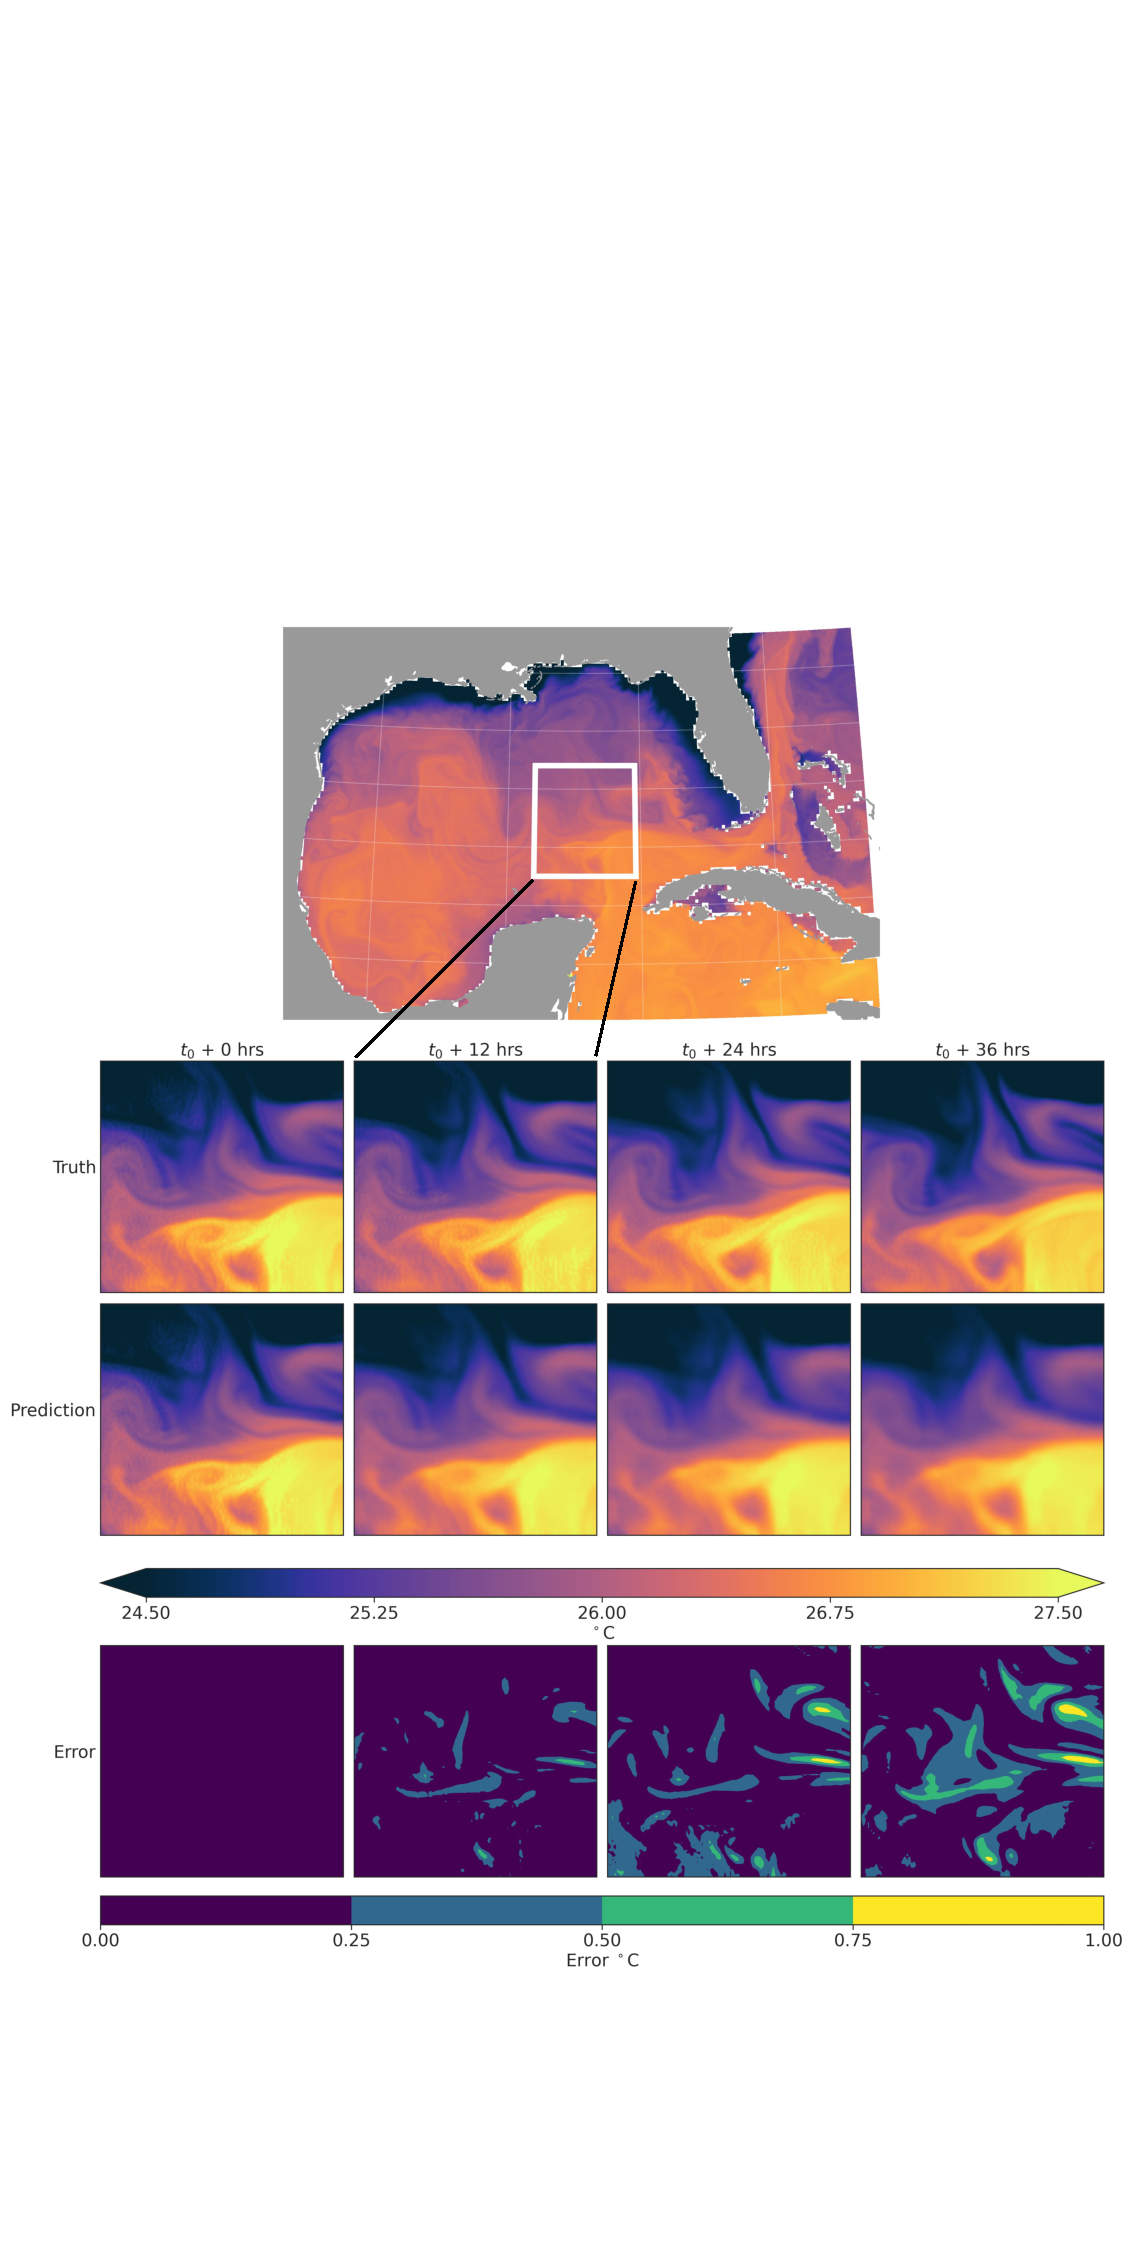
\includegraphics[width=.8\textwidth]{../figures/rc_gom_sst.pdf}
    \caption{A sample prediction of sea surface temperatures in the Gulf of Mexico at 1/25$^\circ$
        horizontal resolution.
        The upper row (Truth) shows the evolution of unseen test data from the
        Navy HYCOM reanalysis product, and the middle row shows a prediction
        from the Echo State Network architecture described in
        \cref{subsec:rc}.
        The bottom row (Error) shows the absolute value of the difference between the two.
        See \cref{sec:gom} for a description of the dataset.
    }
    \label{fig:gom_sst}
\end{figure}

To make the discussion concrete, we present a sample prediction from our own surrogate model
in \cref{fig:gom_sst}.
The panels show the time evolution of Sea Surface Temperature (SST) in the Gulf of Mexico at 1/25$^\circ$ horizontal resolution, using data from a Navy HYCOM, 3D-Var-based reanalysis product as ``Truth'' (upper row; see \cref{sec:gom} for data details).
We generate the prediction (middle row) with an RNN architecture
described more fully in \cref{subsec:rc}.
Generally speaking, the RNN captures the largest scales of the SST pattern over
a 36~hour window.
However, as time progresses, the SST pattern becomes overly smooth.
The RNN is unable to capture the spatial details that are well resolved in the reanalysis
dataset, with the largest errors evolving along sharp SST fronts.
We note that a similar smoothing behavior can be observed in other neural network based emulators, see for example
\citep<>[Figure 1]{bi_pangu-weather_2022},
\citep<>[Figure 4c \& 4d]{pathak_fourcastnet_2022},
\citep<>[Figure 5]{keisler_forecasting_2022}


There are a number of reasons that could cause this smoothing behavior to manifest in the
predictions. One reason is that the training uses a mean-squared error loss function, which is known to prioritize large over
small scale features
\citep{rossa_overview_2008}.
However, we suggest that any blurring effect from such a loss function is exacerbated by more fundamental decisions in the experimental design.
Our primary goal is to explore how temporal subsampling in the training dataset adds to this blurring effect.
We are motivated to study the impact of this subsampling because many existing emulators, including our example in \cref{fig:gom_sst}, rely on reanalysis products as training data
\citep<e.g.>[]{lam_graphcast_2022,bi_pangu-weather_2022,pathak_fourcastnet_2022,keisler_forecasting_2022,weyn_sub-seasonal_2021,arcomano_machine_2020}.
While there are excellent reasons to leverage the existence of reanalysis products, namely that they are constrained to observational data, the shear size of the data requires some
degree of temporal subsampling.
We suggest that it is important to understand how this highly routine data reduction step impacts the performance of data-driven prediction methods when used for training.

In our work, we explore the degree to which temporal subsampling impedes recurrent and autogregressive neural networks from learning the true underlying
dynamics of the system.
In order to isolate this effect from the potential impacts of a data assimilation system and multivariate interactions,  we do not rely on the GoM reanalysis data.
Instead, we use a model for Surface Quasi-Geostrophic (SQG) turbulence
\citep{held_surface_1995}, which additionally
gives us direct control over the datasets used for training, validation, and testing.
The SQG model and dataset generation is described more fully in
\cref{sec:sqg}.

The architectures that we use in this study stem from a broad class of machine learning techniques termed as reservoir computing (RC), which was independently discovered as
Echo State Networks \citep<ESNs;>[]{jaeger_echo_2001},
Liquid State Machines \citep{maass_real-time_2002},
and the Decorrelation Backpropagation Rule
\citep{steil_backpropagation-decorrelation_2004}.
%In our work we employ an Echo State Network architecture, and note the work of
%\citet{verstraeten_experimental_2007}, who presented an empirical unification of
%these techniques.
One defining characteristic of RC models is that all internal connections are adjusted by global or ``macro-scale'' parameters, significantly reducing the
number of parameters that need to be trained.
The relatively simplified structure and training requirements of RC make it an
attractive architecture for large scale prediction because it enables rapid development, and could be useful in situations requiring online learning.
More importantly though, we are motivated to use RC because past studies have repeatedly shown that it can emulate low dimensional chaotic systems while often outperforming more complex RNNs such as those with Long Short-Term Memory units (LSTMs)
\citep<e.g.>[]{platt_systematic_2022,vlachas_backpropagation_2020,griffith_forecasting_2019,lu_attractor_2018,pathak_model-free_2018}.
%and emulate atmospheric dynamics with similar skill as a coarse resolution
%primitive equation GCM \citep{arcomano_machine_2020}.
%Here we summarize a few key results.
%\citet{platt_systematic_2022} showed that by systematically optimizing the RC
%hyperparameters, it can emulate the dynamics of a variety of chaotic systems and
%remain on the ``true'' trajectory out to 4-12 times $1/\lambda_1$ on average, where
%$\lambda_1$ is the leading Lyapunov exponent.
%\citet{pathak_using_2017} and \citet{lu_attractor_2018} showed that when a
%well-calibrated RC model
%eventually diverges from the ``truth'' in a chaotic system, the long-term behavior
%resembles a typical trajectory on the attractor, such that RC respects the
%ergodic properties of the underlying system.
%Moreover, \citet{vlachas_backpropagation_2020} showed that RC can outperform more
%complex RNNs like LSTMs in predicting chaotic dynamics, indicating that the
%fixed internal connections could afford some robustness for prediction.
Additionally, \citet{penny_integrating_2022} showed that RC can be
successfully integrated with a number of data assimilation algorithms, either
by generating samples for ensemble based methods like the Ensemble Kalman Filter,
or by generating the tangent linear model necessary for 4D-Var.
Finally, we note that \citet{gauthier_next_2021} proposed a further
simplification to the RC architecture based on insights from
\citet{bollt_explaining_2021} that unifies versions of RC with nonlinear vector autoregression (NVAR).
For a variety of chaotic systems, this architecture has shown excellent prediction skill
even with low order, polynomial-based feature vectors
\citep{chen_next_2022,barbosa_learning_2022,gauthier_next_2021}, despite requiring a much
smaller hidden state and less training data.
Considering all of these advancements, in addition to studying the effect of temporal subsampling on emulator performance, a secondary goal of this work is to show how well the simple yet powerful single-layer NVAR and ESN architectures perform in emulating turbulent geophysical fluid dynamics (see \cref{sec:rnn-architecture} for architecture
details).

%In this work, we probe the following questions more precisely:
%\begin{itemize}
%    \item What spatial scales can be resolved by NN emulators?
%    \item How do fundamental choices in the training data, like temporal
%        subsampling or spatial rescaling, impact the prediction skill?
%    \item How do architectural changes to the network impact prediction skill?
%\end{itemize}
%In the study, we use two forms of RNNs to emulate dynamics relevant to
%geophysical fluids: Reservoir Computing (RC) and a form of Nonlinear Vector
%Autoregression (NVAR) that is motivated by the RC paradigm (described
%in \cref{sec:rnn-architecture}).
%Throughout the study, we focus our attention on how well these RNNs can emulate
%turbulent Surface
%Quasi-Geostrophic (SQG) motion (\cref{sec:sqg}).
%We show in \cref{sec:results} that this relatively idealized model exhibits similar
%smoothing behavior as shown in the Gulf of Mexico SST prediction.
%However, using this model allows us to quantify the resolved scales of motion
%more readily, and make changes to the training data, so that we can address the
%questions outlined above.
%While of course we cannot test all NN architectures for emulating these
%dynamics, we discuss the broader implications of our RNN-based results
%for the general setting of NN emulation development for weather and climate
%prediction in \cref{sec:discussion}.
